\section{Bar chart, line chart}

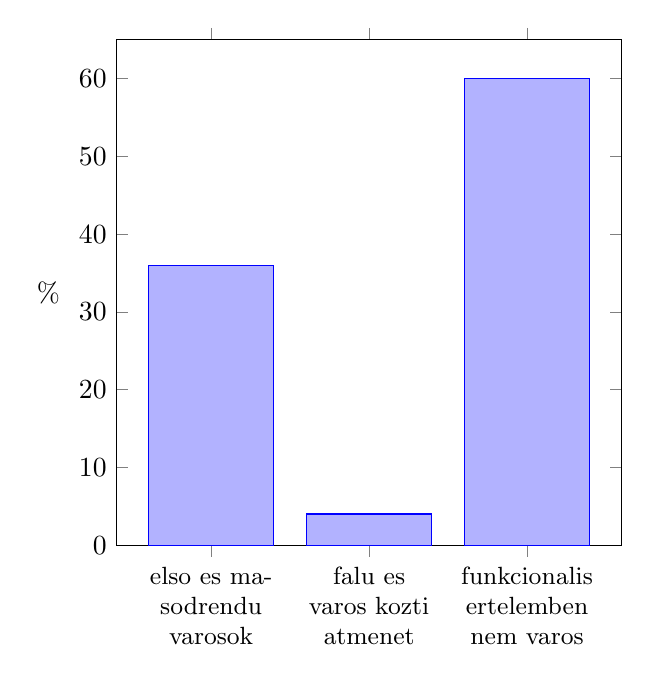
\begin{tikzpicture}
\begin{axis}[
             width=8cm,
             height=8cm,
             symbolic x coords={elso es masodrendu varosok,
                                falu es varos kozti atmenet,
                                funkcionalis ertelemben nem varos},
             x tick label style={font=\small,text width=1.7cm,align=center},
             xtick=data,
             ymin=0,
             ymax=65,
             ylabel=\%,
             ylabel style={rotate=-90},
             ybar,
             enlarge x limits=.3,
             bar width=45pt,
             ]
\addplot coordinates {
                      (elso es masodrendu varosok,36)
                      (falu es varos kozti atmenet,4)
                      (funkcionalis ertelemben nem varos,60)};
\end{axis}
\end{tikzpicture}

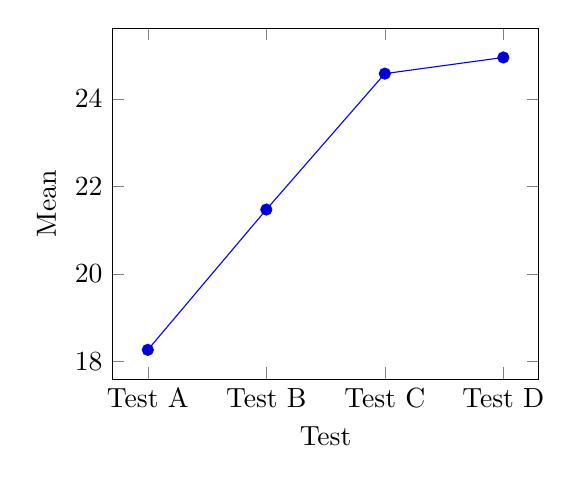
\begin{tikzpicture}
    \begin{axis}
        [
        ,width=7cm
        ,xlabel=Test
        ,ylabel=Mean
        ,xtick=data,
       %,xtick={0,1,...,3}
        ,xticklabels={Test A,Test B,Test C,Test D}
        ]
        \addplot+[sharp plot] coordinates
        {(0,18.26) (1,21.47) (2,24.58) (3,24.95)};
    \end{axis}
\end{tikzpicture}

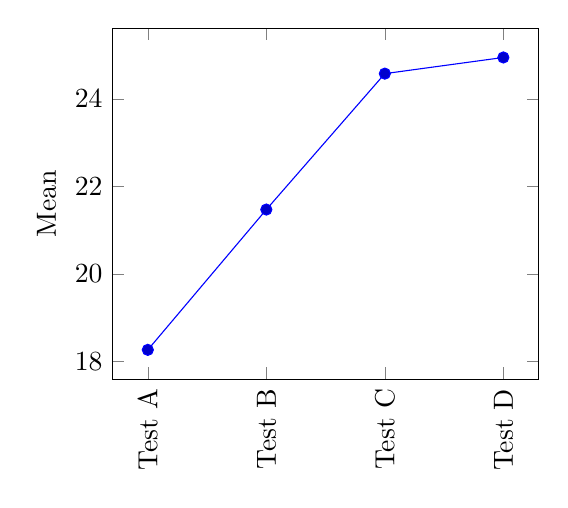
\begin{tikzpicture}
    \begin{axis}
        [
        width=7cm,
        %xlabel=Test,
        ylabel=Mean,
        xtick=data,
        xticklabels={Test A,Test B,Test C,Test D},
        x tick label style={rotate=90,anchor=east}
        ]
        \addplot+[sharp plot] coordinates
        {(0,18.26) (1,21.47) (2,24.58) (3,24.95)};
    \end{axis}
\end{tikzpicture}
